\documentclass[twocolumn]{article}
\usepackage[T1]{fontenc}
\usepackage[utf8]{inputenc}
\usepackage{tabularx,ragged2e,booktabs,caption}
\usepackage{multirow}
\usepackage{color}
\usepackage[top=1in,bottom=1in,left=1.2in,right=1.2in]{geometry}
\usepackage{hyperref}
\usepackage[small]{titlesec}
\usepackage{cite}
\usepackage{graphicx}

\renewcommand\tabularxcolumn[1]{C{#1}}

\newcommand{\todo}[1]{\textcolor{cyan}{\textbf{TODO:} #1}}

\title{CS378: Final Project - Data Artifacts \\ \url{https://github.com/sarimaleem/cs378_fp}}
\author{Sarim Aleem \\ ska2222}

\date{}

\begin{document}
\maketitle


\begin{abstract}
    \todo{write an abstract describing the core motivation and findings from your project}
\end{abstract}

\section{Introduction (5pt)}

\todo{This section should include three paragraphs. The first paragraph is to
briefly describe task and data. The second paragraph should describe the
results of your analysis, and the third paragraph describing your fix and main
experimental take aways. }

The model that was used was \cite{clark2020electra}


\section{Task/Dataset/Model Description (15pt)}

\todo{Describe the task/dataset/model you are working on. Clearly define your
task with mathematical notations. Describe your learning algorithm. You must
formally specify the loss function, stopping criteria, training data, etc used
for the model you are analyzing in the next section. Remember, every notation
you use must be defined.}

\section{Performance Analysis (25pt)}

The model was trained for 3 iterations on the SNLI training dataset. Each
iteration has 550152 training examples, the batch size for the training examples
was 32. All training was done on google colab in the cloud, and training took
about 25 minutes.

\subsection*{Overall Accuracy Statistics}

An initial evaluation of the model shows that it has an accuracy of 88\%. We
also did further evaluation to show statistics about which labels it
misclassified most using a confusion matrix.

\begin{table}[]
\caption{Development Set Evaluation Metrics}
\centering
\begin{tabular}{|l|l|}
\hline
loss       & 0.315   \\ \hline
accuracy   & 0.8865  \\ \hline
runtime    & 20.2629 \\ \hline
examples/s & 485.715 \\ \hline
steps/s    & 60.751  \\ \hline
\end{tabular}
\caption*{\textit{Model Metrics for 9842 examples}}

\caption{Confusion Matrix}
\begin{tabular}{|c|cccc|c|}
\hline
\multicolumn{1}{|l|}{}         & \multicolumn{4}{c|}{\textbf{Predicted}}                                                                              & \multicolumn{1}{l|}{} \\ \hline
\multirow{4}{*}{\textbf{True}} & \multicolumn{1}{l|}{}               & \multicolumn{1}{c|}{\textit{0}} & \multicolumn{1}{c|}{\textit{1}} & \textit{2} & \textbf{Total}        \\ \cline{2-6} 
                               & \multicolumn{1}{c|}{\textit{0}}     & \multicolumn{1}{c|}{2996}       & \multicolumn{1}{c|}{252}        & 81         & 3329                  \\ \cline{2-6} 
                               & \multicolumn{1}{c|}{\textit{1}}     & \multicolumn{1}{c|}{213}        & \multicolumn{1}{c|}{2787}       & 235        & 3235                  \\ \cline{2-6} 
                               & \multicolumn{1}{c|}{\textit{2}}     & \multicolumn{1}{c|}{79}         & \multicolumn{1}{c|}{257}        & 2942       & 3278                  \\ \hline
\multicolumn{1}{|l|}{}         & \multicolumn{1}{c|}{\textbf{Total}} & \multicolumn{1}{c|}{3288}       & \multicolumn{1}{c|}{3296}       & 3258       & \textbf{9842}         \\ \hline
\end{tabular}
\caption*{\textit{ 0=Entailment, 1=Neutral, 2=Contradiction }}

\caption{Percent mispredictions}
\begin{tabular}{|l|cccc|}
\hline
                               & \multicolumn{4}{c|}{\textbf{Predicted}}                                                                          \\ \hline
\multirow{4}{*}{\textbf{True}} & \multicolumn{1}{l|}{}           & \multicolumn{1}{c|}{\textit{0}} & \multicolumn{1}{c|}{\textit{1}} & \textit{2} \\ \cline{2-5} 
                               & \multicolumn{1}{c|}{\textit{0}} & \multicolumn{1}{c|}{89.99}      & \multicolumn{1}{c|}{7.78}       & 2.47       \\ \cline{2-5} 
                               & \multicolumn{1}{c|}{\textit{1}} & \multicolumn{1}{c|}{6.39}       & \multicolumn{1}{c|}{86.15}      & 7.16       \\ \cline{2-5} 
                               & \multicolumn{1}{c|}{\textit{2}} & \multicolumn{1}{c|}{2.37}       & \multicolumn{1}{c|}{7.94}       & 89.74      \\ \hline
\end{tabular}
\caption*{\textit{ 0=Entailment, 1=Neutral, 2=Contradiction }}
\end{table}

\subsection{Confusion Matrix Analysis}
In general, the model seems to do well with Separating Entailment and
Contradiction. For example, it only incorrectly identifies 2.47\% of entailment
examples as contradiction and 2.37\% of contradiction examples as entailement.

However, the model struggles more to understand the relationship between,
entailment and neutral, as well as contradiction and neutral. For example, it
mispredicted over 7\% of entailments and contradictions as neutrals. As long as 
mispredicting over 6\% of neutrals as entailments and over 7\% of of neutrals as
contradictions.

\subsection{Manual Pattern Analysis}

It's difficult to say how the model is evaluating sentences, since it's
impossible to fully understand its weights. Nevertheless, there do seem to be
some patterns one evaluating mistakes that the model makes. One pattern that
seems to happen is that the model seems to be unable to understand different
words that mean the same thing in a context. For example, the following is an
error that the model made. 

In the example with hypothesis \textit{A man and a woman are looking at produce
on display} and premise \textit{A man and woman are staring at heads of
lettuce}. The model is unable to distinguish that lettuce is a type of produce
and instead makes assumption that they are different, thus leading it to think
they are contradictions.

\begin{table*}[t]
\caption{Examples of model misunderstanding words, or not considering their importance}
\begin{tabular}{|p{4cm}|p{4cm}|p{2.5cm}|p{2.5cm}|}
\hline
\textbf{premise}                                                                        & \textbf{Hypothesis}                & \textbf{Gold} & \textbf{Predicted} \\ \hline
People are throwing tomatoes at each other                                                                    & The people are having a food fight               & entailment                         & contradiction      \\ \hline
A man and a woman are looking at produce on display.                                                          & A man and women are staring at heads of lettuce. & neutral                            & contradiction      \\ \hline
Two men sitting on a subway are reading, with coats and scarves on, but have seemed to have lost their pants. & The men are wearing pants.                       & contradiction                      & entailment         \\ \hline
Two men are in an electronics workshop, working on computers or equipment                                     & The men are unaware of what computers are.       & contradiction                      & neutral            \\ \hline
\end{tabular}
\end{table*}


\subsection{Using Contast sets to evaluate the Model}
subsection{Contrast Sets}

In their article \textit{Evaluating models' local decision boundaries via
contrast sets} \cite{gardner2020evaluating}, Gardner et al. explain the concept
of a \textit{contrast set}. A contrast set is a small but meaninful alteration
in the input data that typically leads to a different gold label.

In order to test if the model is finding artifacts in the data or genuinely
evaluating it, we annotated 35 different examples in the validation data that
the model predicted correctly, and then tested to see if the model was able to
predict them correctly again.

The results of the model showed a significant dip in accuracy, with accuracy
going down to 77\% from 89\%. The model mispredicted 8/35 examples. One pattern
that emerged from the mispredictions is that the model fails to see correlations
between various words and also fails to understand the relationships between
various words. The following is an example of this phenomenon: \\

\begin{quote}
premise: Two men on vehicles competing in a race. \\
hypothesis: Men are riding cars on the street. \\
label: neutral \\
predicted: contradiction
\end{quote}

The neural network is essentially unable to distinguish that different words can
have the same meaning (in this case vehicles and cars).

\section{Describing Your Fix (20pt)}

It is clear that the issue with the model is that it fails to understand
ambiguous training examples. This is especially seen given that the model
largely confuses, as seen earlier, neutral and entailment and instances of
contradiction. 


\begin{figure}
  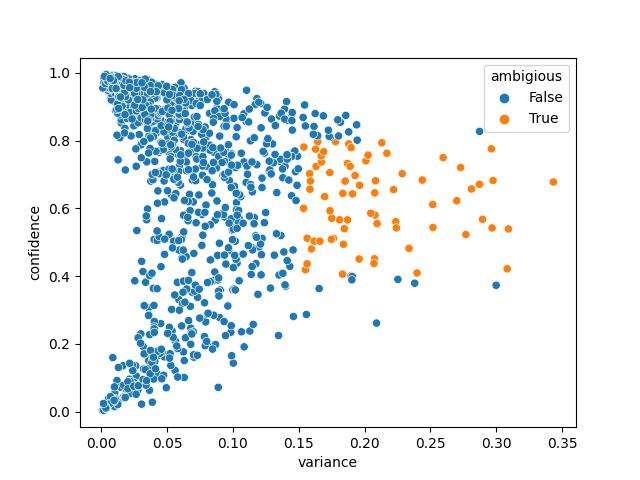
\includegraphics[width=\linewidth]{./ambiguous.jpg}
  \caption{Data Cartogram of 2000 training examples}
  \label{}
\end{figure}

\subsection{Dataset Cartography}

Training on labels that are ambiguous, that have high variablity, should in
theory help with this issue, even more so than hard to learn labels. An
ambiguous label is defined as a label that has high variance when predicted by
different iterations of the model. For example, a model that is trained on 500
iterations would predict the input differently than a model trained with 1000
iterations or a model trained with 1500 iterations. Furthermore, the average
confidence of that training example is not high or low.
\cite{swayamdipta2020dataset} We reproduced the code to analyze data, and have
plotted 500 training examples in figure 1. 

In order to deal with this, we first created a program that finds ambiguous
examples. We found the variance of the training example based on its confidence
of the gold label from a modeled trained on 500 iterations, 1000 iterations,
1500 iterations, 2000 iterations, 2500 iterations, and 3000 iterations. If th
variance was greater than 0.2, and the confidence of the model was in between
0.6 and 0.7, the example was deemed ambiguous. According to \textit{Swayamdipta
et al.}, training solely ambiguous examples leads to to greater performance
than training on the whole dataset, only easy to learn examples, or only hard to
learn examples. Thus it is logical to train on these examples. 

We pulled 1655 ambiguous samples from the training data and trained on those examples.

\section{Evaluating Your Fix (25pt)}


\todo{
Your writeup should address how effective is your fix, how broadly applicable
is your fix, etc. Providing a single number (overall accuracy) is necessary but
not sufficient here. For example, if your change made the model better on
challenging NLI examples, you could try to quantify that on one or more slices
of the data, give examples of predictions that are fixed, or even use model
interpretation techniques to try to support claims about how your improved
model is doing its ``reasoning.'' (You can look at the papers listed above to
get a sense of how to do such fine-grained evaluation).  You should report
results from a baseline approach (your initial trained model) as well as your
``best'' method. If doing your own project, baselines such as majority class,
random, or a linear classifier are important to see. \textbf{Ablations}: If you
tried several things, analyze the contribution from each one. These should be
\emph{minimal} changes to the same system; try running things with just one
aspect different in order to assess how important that aspect is. This part of
the report should be at least one page.}


% \todo{Describe the data you use, including how many examples are in the training, development, and test sets. Please also provide shallow statistics of your data, with at least the vocabulary size and instruction length. It is best to report all the statistics, including counts, in a table. Please describe how you compute statistics that can be computed in different ways (i.e., vocabulary size). Describe how you pre-process the data, including how you treat casing, tokenization, unknown words, and anything else that you did to the raw data before providing it to your model. If you are using a subset of the data, explain why and discuss tradeoffs (you will also need to back them with experiments).}

% \section{Implementation Details (3pt)}

% \todo{Briefly describe the implementation details. No need to copy details already specified in the assignment. Include any hyper-parameters the model has. If there are any optimizations that you introduced, this is the place to describe them. Did you have to do any special optimizations to make the method work in reasonable time/memory? Describe it here.}

% \section{}

 \section{Related Work (5pt)}
\todo{Briefly discuss prior research papers related to your approach. This will
likely some papers in the project description document. How is your approach
different from existing studies?}
% \paragraph{Ablations (15pt)}

% \todo{Please report your ablation studies on the development set. Make sure to ablate each feature set independently to show they contribute to your final result.  If a feature set does not improve performance, please do not include it -- it doesn't help. You can still discuss it, but there is really no point in including it in your final model. Reporting the results must be done in a table, and each result must be discussed in the text.}

% \section{Error Analysis (7pt)}

% \todo{Qualitative analysis of selected failure examples. Show and discuss error examples from your development set. You must identify certain classes of errors and use the examples to illustrate them. This is often best to show in a table.}

\section{Conclusion (5pt)}
\todo{Brief conclusion summarizing findings from both numerical results and
qualitative analysis.}

\section*{(Optional) AI Assistance}

\todo{If you have used any AI toolkit (either for writing assistance or code
assistance) for your final project, please describe it here. }

\bibliography{sample}{}
\bibliographystyle{plain}


\end{document}
